% Options for packages loaded elsewhere
\PassOptionsToPackage{unicode}{hyperref}
\PassOptionsToPackage{hyphens}{url}
%
\documentclass[
]{book}
\usepackage{amsmath,amssymb}
\usepackage{lmodern}
\usepackage{iftex}
\ifPDFTeX
  \usepackage[T1]{fontenc}
  \usepackage[utf8]{inputenc}
  \usepackage{textcomp} % provide euro and other symbols
\else % if luatex or xetex
  \usepackage{unicode-math}
  \defaultfontfeatures{Scale=MatchLowercase}
  \defaultfontfeatures[\rmfamily]{Ligatures=TeX,Scale=1}
\fi
% Use upquote if available, for straight quotes in verbatim environments
\IfFileExists{upquote.sty}{\usepackage{upquote}}{}
\IfFileExists{microtype.sty}{% use microtype if available
  \usepackage[]{microtype}
  \UseMicrotypeSet[protrusion]{basicmath} % disable protrusion for tt fonts
}{}
\makeatletter
\@ifundefined{KOMAClassName}{% if non-KOMA class
  \IfFileExists{parskip.sty}{%
    \usepackage{parskip}
  }{% else
    \setlength{\parindent}{0pt}
    \setlength{\parskip}{6pt plus 2pt minus 1pt}}
}{% if KOMA class
  \KOMAoptions{parskip=half}}
\makeatother
\usepackage{xcolor}
\usepackage{color}
\usepackage{fancyvrb}
\newcommand{\VerbBar}{|}
\newcommand{\VERB}{\Verb[commandchars=\\\{\}]}
\DefineVerbatimEnvironment{Highlighting}{Verbatim}{commandchars=\\\{\}}
% Add ',fontsize=\small' for more characters per line
\usepackage{framed}
\definecolor{shadecolor}{RGB}{248,248,248}
\newenvironment{Shaded}{\begin{snugshade}}{\end{snugshade}}
\newcommand{\AlertTok}[1]{\textcolor[rgb]{0.94,0.16,0.16}{#1}}
\newcommand{\AnnotationTok}[1]{\textcolor[rgb]{0.56,0.35,0.01}{\textbf{\textit{#1}}}}
\newcommand{\AttributeTok}[1]{\textcolor[rgb]{0.77,0.63,0.00}{#1}}
\newcommand{\BaseNTok}[1]{\textcolor[rgb]{0.00,0.00,0.81}{#1}}
\newcommand{\BuiltInTok}[1]{#1}
\newcommand{\CharTok}[1]{\textcolor[rgb]{0.31,0.60,0.02}{#1}}
\newcommand{\CommentTok}[1]{\textcolor[rgb]{0.56,0.35,0.01}{\textit{#1}}}
\newcommand{\CommentVarTok}[1]{\textcolor[rgb]{0.56,0.35,0.01}{\textbf{\textit{#1}}}}
\newcommand{\ConstantTok}[1]{\textcolor[rgb]{0.00,0.00,0.00}{#1}}
\newcommand{\ControlFlowTok}[1]{\textcolor[rgb]{0.13,0.29,0.53}{\textbf{#1}}}
\newcommand{\DataTypeTok}[1]{\textcolor[rgb]{0.13,0.29,0.53}{#1}}
\newcommand{\DecValTok}[1]{\textcolor[rgb]{0.00,0.00,0.81}{#1}}
\newcommand{\DocumentationTok}[1]{\textcolor[rgb]{0.56,0.35,0.01}{\textbf{\textit{#1}}}}
\newcommand{\ErrorTok}[1]{\textcolor[rgb]{0.64,0.00,0.00}{\textbf{#1}}}
\newcommand{\ExtensionTok}[1]{#1}
\newcommand{\FloatTok}[1]{\textcolor[rgb]{0.00,0.00,0.81}{#1}}
\newcommand{\FunctionTok}[1]{\textcolor[rgb]{0.00,0.00,0.00}{#1}}
\newcommand{\ImportTok}[1]{#1}
\newcommand{\InformationTok}[1]{\textcolor[rgb]{0.56,0.35,0.01}{\textbf{\textit{#1}}}}
\newcommand{\KeywordTok}[1]{\textcolor[rgb]{0.13,0.29,0.53}{\textbf{#1}}}
\newcommand{\NormalTok}[1]{#1}
\newcommand{\OperatorTok}[1]{\textcolor[rgb]{0.81,0.36,0.00}{\textbf{#1}}}
\newcommand{\OtherTok}[1]{\textcolor[rgb]{0.56,0.35,0.01}{#1}}
\newcommand{\PreprocessorTok}[1]{\textcolor[rgb]{0.56,0.35,0.01}{\textit{#1}}}
\newcommand{\RegionMarkerTok}[1]{#1}
\newcommand{\SpecialCharTok}[1]{\textcolor[rgb]{0.00,0.00,0.00}{#1}}
\newcommand{\SpecialStringTok}[1]{\textcolor[rgb]{0.31,0.60,0.02}{#1}}
\newcommand{\StringTok}[1]{\textcolor[rgb]{0.31,0.60,0.02}{#1}}
\newcommand{\VariableTok}[1]{\textcolor[rgb]{0.00,0.00,0.00}{#1}}
\newcommand{\VerbatimStringTok}[1]{\textcolor[rgb]{0.31,0.60,0.02}{#1}}
\newcommand{\WarningTok}[1]{\textcolor[rgb]{0.56,0.35,0.01}{\textbf{\textit{#1}}}}
\usepackage{longtable,booktabs,array}
\usepackage{calc} % for calculating minipage widths
% Correct order of tables after \paragraph or \subparagraph
\usepackage{etoolbox}
\makeatletter
\patchcmd\longtable{\par}{\if@noskipsec\mbox{}\fi\par}{}{}
\makeatother
% Allow footnotes in longtable head/foot
\IfFileExists{footnotehyper.sty}{\usepackage{footnotehyper}}{\usepackage{footnote}}
\makesavenoteenv{longtable}
\usepackage{graphicx}
\makeatletter
\def\maxwidth{\ifdim\Gin@nat@width>\linewidth\linewidth\else\Gin@nat@width\fi}
\def\maxheight{\ifdim\Gin@nat@height>\textheight\textheight\else\Gin@nat@height\fi}
\makeatother
% Scale images if necessary, so that they will not overflow the page
% margins by default, and it is still possible to overwrite the defaults
% using explicit options in \includegraphics[width, height, ...]{}
\setkeys{Gin}{width=\maxwidth,height=\maxheight,keepaspectratio}
% Set default figure placement to htbp
\makeatletter
\def\fps@figure{htbp}
\makeatother
\setlength{\emergencystretch}{3em} % prevent overfull lines
\providecommand{\tightlist}{%
  \setlength{\itemsep}{0pt}\setlength{\parskip}{0pt}}
\setcounter{secnumdepth}{5}
\usepackage{booktabs}
\usepackage{amsthm}
\makeatletter
\def\thm@space@setup{%
  \thm@preskip=8pt plus 2pt minus 4pt
  \thm@postskip=\thm@preskip
}
\makeatother
\usepackage{booktabs}
\usepackage{longtable}
\usepackage{array}
\usepackage{multirow}
\usepackage{wrapfig}
\usepackage{float}
\usepackage{colortbl}
\usepackage{pdflscape}
\usepackage{tabu}
\usepackage{threeparttable}
\usepackage{threeparttablex}
\usepackage[normalem]{ulem}
\usepackage{makecell}
\usepackage{xcolor}
\ifLuaTeX
  \usepackage{selnolig}  % disable illegal ligatures
\fi
\usepackage[]{natbib}
\bibliographystyle{apalike}
\IfFileExists{bookmark.sty}{\usepackage{bookmark}}{\usepackage{hyperref}}
\IfFileExists{xurl.sty}{\usepackage{xurl}}{} % add URL line breaks if available
\urlstyle{same} % disable monospaced font for URLs
\hypersetup{
  pdftitle={Half-day Workshop on Phylogenetic Comparative Methods},
  pdfauthor={Simon Joly},
  hidelinks,
  pdfcreator={LaTeX via pandoc}}

\title{Half-day Workshop on Phylogenetic Comparative Methods}
\author{Simon Joly}
\date{2023-02-10}

\begin{document}
\maketitle

{
\setcounter{tocdepth}{1}
\tableofcontents
}
\hypertarget{preface}{%
\chapter{Preface}\label{preface}}

This document consist in an introduction to the comparative methods. It contains theory as well as practical examples in R on Phylogenetic Generalized Least Squares (PGLS). It was developed for a half-day workshop that consists in short presentations followed by R exercises. Note that the present document should pretty much stand by itself because most of the theory given in the presentations are incorporated into the theory sections. Therefore, this document should contain all the necessary information to understand the examples.

I assume that the readers are ``reasonably'' familiar with R as well as with linear regression and its assumptions. There are a lot of good R introductory tutorials on the web and for linear models. Zuur et al.~(2007) provide a good introduction to linear models, mixed-effects models and model comparison. Good introductions to model fitting in R can also be found on Dolph Schluter's \href{https://www.zoology.ubc.ca/~schluter/R/fit-model/}{webpage} and among the \href{http://qcbs.ca/wiki/r_workshop4}{QCBS workshops}.

\hypertarget{other-useful-information}{%
\chapter{Other useful information}\label{other-useful-information}}

The links below might provide additional information of interest.

\href{https://lukejharmon.github.io/pcm/}{Luke Harmon's book - Phylogenetic Comparative Methods}

\href{http://github.com/simjoly/CourseComparativeMethods/}{Course on Phylogenetic Comparative Methods}

\href{http://htmlpreview.github.com/?http://github.com/simjoly/CourseComparativeMethods/blob/master/lecture1/Introduction_phylo.html}{Introduction to phylogenies in R} - \href{http://github.com/simjoly/CourseComparativeMethods/blob/master/lecture1/Introduction_phylo.pdf}{pdf}

\href{http://htmlpreview.github.com/?http://github.com/simjoly/CourseComparativeMethods/blob/master/lecture2/PhylogeneticTree.html}{Reading and making phylogenetic trees in R} - \href{http://github.com/simjoly/CourseComparativeMethods/blob/master/lecture2/PhylogeneticTree.pdf}{pdf}

\hypertarget{disclaimer}{%
\chapter{Disclaimer}\label{disclaimer}}

This tutorial is provided as is, without any guaranty that it will work or that the analyses will be up to date.

\hypertarget{before}{%
\chapter{Ahead of the workshop}\label{before}}

Here are a few things you should know and you should do ahead of the workshop.

\hypertarget{install-r-and-the-required-packages}{%
\section{Install R and the required packages}\label{install-r-and-the-required-packages}}

To perform the examples of this document, you will need to have the \href{https://www.r-project.org/}{R software} installed on your computer. I also recommend that you install \href{https://rstudio.com/}{RStudio}. If R Studio is not required, it facilitates interactions between scripts and the R console and provides many great tools.

After installing R, you will have to install some packages. For this specific tutorial, we will need to load the following R packages.

\begin{Shaded}
\begin{Highlighting}[]
\FunctionTok{library}\NormalTok{(nlme)}
\FunctionTok{library}\NormalTok{(ape)}
\FunctionTok{library}\NormalTok{(RColorBrewer)}
\FunctionTok{library}\NormalTok{(ggplot2)}
\end{Highlighting}
\end{Shaded}

To execute the code of this tutorial in R, you can just copy and paste the code in the boxes in your R console. This will replicate the analyses presented in the tutorial.

If some of the packages above are not yet installed on your computer, you get error messages when trying to load them. If this is the case, you will have to install them using the function \texttt{install.packages()}. You only have to install them only once.

\begin{Shaded}
\begin{Highlighting}[]
\FunctionTok{install.packages}\NormalTok{(}\StringTok{\textquotesingle{}nlme\textquotesingle{}}\NormalTok{)}
\FunctionTok{install.packages}\NormalTok{(}\StringTok{\textquotesingle{}ape\textquotesingle{}}\NormalTok{)}
\FunctionTok{install.packages}\NormalTok{(}\StringTok{\textquotesingle{}RColorBrewer\textquotesingle{}}\NormalTok{)}
\FunctionTok{install.packages}\NormalTok{(}\StringTok{\textquotesingle{}ggplot2\textquotesingle{}}\NormalTok{)}
\end{Highlighting}
\end{Shaded}

Once the packages are installed, you can load the packages using the \texttt{library()} function. Also note that if you are using both the packages \texttt{nlme} and \texttt{ape}, \texttt{nlme} should be loaded first. If you don't do this, you might get errors; you could then restart R and start over.

\hypertarget{working-with-github}{%
\section{Working with github}\label{working-with-github}}

All the data of the workshop are deposited in a github repository. The easiest way to access them is to go to the \href{http://www.github.com/simjoly/ComparativeMethods-HalfDayWorkshop}{Workshop repository} and clone it on your computer. The option to clone the directory is in a green box called ``code''.

Once you have cloned the repository, you need to open R (R studio) and set the working directory to the repository folder (``/ComparativeMethods-HalfDayWorkshop''). In RStudio, to change the working directory, you choose \texttt{\textgreater{}Session\textgreater{}Set\ Working\ directory\textgreater{}Choose\ Directory}.You are now ready for the workshop.

\hypertarget{intro}{%
\chapter{An introduction to Phylogenetic Comparative Methods}\label{intro}}

Phylogenetic comparative methods were introduced by Joseph Felsenstein in 1985. The idea of phylogenetic comparative methods was to correct for the non-independence of species in statistical tests because of their shared evolutionary histories. Indeed, two species may look similar not because they live in the same environment but because they are closely related. For instance, considering the following angiosperm phylogeny.

\begin{figure}

{\centering 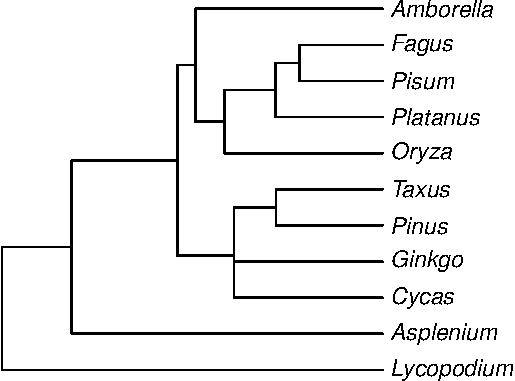
\includegraphics{bookdown-demo_files/figure-latex/AngiospermTree-1} 

}

\caption{land plant phylogeny}\label{fig:AngiospermTree}
\end{figure}

It is clear that \emph{Fagus} (beech) and \emph{Pisum} (pea) are more likely to share similar characteristics compared to \emph{Asplenium} (a fern), because they share a more recent common ancestor. In other words, their evolutionary histories are shared over a longer period than with \emph{Asplenium}. As such, they have more chance to have more similar traits (and in fact they do). For instance, take two characters, ovule and fertilization type, within this group.

\begin{center}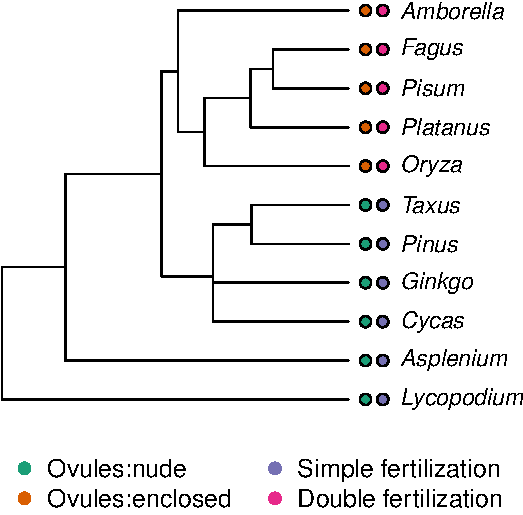
\includegraphics{bookdown-demo_files/figure-latex/AngiospermsWithCharacters-1} \end{center}

Ignoring the phylogeny, we might be tempted to see a strong correlation between these two characters. Indeed, the states between the two characters show a perfect correspondence. Using standard contingency table statistics, we could do a Fisher exact test:

\begin{Shaded}
\begin{Highlighting}[]
\FunctionTok{fisher.test}\NormalTok{(}\FunctionTok{matrix}\NormalTok{(}\FunctionTok{c}\NormalTok{(}\DecValTok{5}\NormalTok{,}\DecValTok{0}\NormalTok{,}\DecValTok{0}\NormalTok{,}\DecValTok{6}\NormalTok{),}\AttributeTok{ncol=}\DecValTok{2}\NormalTok{))}
\end{Highlighting}
\end{Shaded}

\begin{verbatim}
## 
##  Fisher's Exact Test for Count Data
## 
## data:  matrix(c(5, 0, 0, 6), ncol = 2)
## p-value = 0.002165
## alternative hypothesis: true odds ratio is not equal to 1
## 95 percent confidence interval:
##  2.842809      Inf
## sample estimates:
## odds ratio 
##        Inf
\end{verbatim}

The test suggests that the assotiation is highly significant. However, we know that the comparisons made are not completely independent. Actually, both characters evolved only once, and this along the same branch.

A more appropriate question would be ``what is the probability that two characters evolved along the same branch?''. This can be calculated using a contingency table, but this time taking the observations along the branches of the phylogeny. In the example, there are 18 branches and the two characters evolved only once and on the same branch. The contingency table when considering the changes along the branches looks like this:

\begin{tabular}{>{}l|r|r}
\hline
  & Change in trait 2 & No change in trait 2\\
\hline
\textbf{Change in trait 1} & 1 & 0\\
\hline
\textbf{No change in trait 1} & 0 & 17\\
\hline
\end{tabular}

With this table, Fisher's exact test will give the following result:

\begin{Shaded}
\begin{Highlighting}[]
\FunctionTok{fisher.test}\NormalTok{(}\FunctionTok{matrix}\NormalTok{(}\FunctionTok{c}\NormalTok{(}\DecValTok{1}\NormalTok{,}\DecValTok{0}\NormalTok{,}\DecValTok{0}\NormalTok{,}\DecValTok{17}\NormalTok{),}\AttributeTok{ncol=}\DecValTok{2}\NormalTok{))}
\end{Highlighting}
\end{Shaded}

\begin{verbatim}
## 
##  Fisher's Exact Test for Count Data
## 
## data:  matrix(c(1, 0, 0, 17), ncol = 2)
## p-value = 0.05556
## alternative hypothesis: true odds ratio is not equal to 1
## 95 percent confidence interval:
##  0.4358974       Inf
## sample estimates:
## odds ratio 
##        Inf
\end{verbatim}

You can see that the result is no longer significant. While this approach is correct, more powerful comparative methods have been developped. One useful and powerful approach is the Phylogenetic Generalized Least Squares (PGLS) and it is the one that will be introduced next. But first, let's do some revision and look briefly at the standard regression to better understand PGLS.

  \bibliography{book.bib}

\end{document}
